\documentclass[spanish, a4paper, 12pt] {article}
\usepackage[spanish]{babel}
\usepackage[utf8]{inputenc}
\usepackage{amsmath}
\usepackage{amssymb}
\usepackage{amsfonts}
\usepackage{latexsym}
\usepackage{mathtools}
\usepackage{anysize}
%\marginsize{2cm}{2cm}{2cm}{3cm}
\newcommand\eqdef{\stackrel{\mathclap{\mbox{\tiny{def}}}}{=}}
\newcommand\eqac{\stackrel{\mathclap{\mbox{*}}}{=}}

\usepackage{graphicx}
\usepackage{hyperref}
\usepackage{float}
\usepackage{verbatim}
\DeclareGraphicsExtensions{.pdf,.png,.jpg}

\usepackage[a4paper,bindingoffset=0.2in,left=0.8in,right=0.8in,top=1.1in,bottom=1in,footskip=.25in]{geometry}

\begin{document}
\title{\vspace{-1.75cm}Entrega 1}
\author{Marco Antonio Garrido Rojo\thanks{\url{https://github.com/MaSteve/EDIF} Esta entrega puede encontrarse en GitHub.}\vspace{-0.5cm}}
\date{\vspace{-0.5cm}}
\maketitle
\vspace{-0.25cm}
Sea la función $g(x) = 5x^{\frac{4}{5}}$ a lo largo del ejercicio.
\begin{itemize}
\item{
\textbf{Apartado 1} Estudia la continuidad y derivabilidad de la función $g(x), x \in \mathbb{R}$. Determinar si es lipschitziana en algún intervalo $[-r, r], r > 0$.

La continuidad de esta función se justifica rápidamente por composición de funciones continuas (elevar a la cuarta es continua en todo $\mathbb{R}$, la raiz quinta no da problemas en $\mathbb{R}^{+} \cup \{0\}$ y el producto por escalares tampoco).

La derivabilidad tiene algo más de gracia. $g'(x) = \frac{4}{\sqrt[5]{x}}$ que claramente no está definida en el cero, donde cuenta con una asíntota.

Visto esto último, la función claramente no puede ser lipschitziana en ese intervalo porque, apoyándonos en la definición de derivada y en que esta no está acotada para $g(x)$, tenemos que $\forall \varepsilon > 0$, $\exists \delta > 0$ $/$ $\forall x_0 \in I$, $|x_0 - x| < 0 \Rightarrow |\frac{g(x_0)-g(x)}{x_0 - x} - g'(x)| < \varepsilon$ donde $x$ lo cogemos distinto de $0$ pero lo suficientemente cercano a este valor para que $|g'(x)| > K + \varepsilon$, donde $K$ sería una supuesta constante de Lipschitz que fracasa para cualquier valor positivo.
$\hfill \square$
}
\item{
\textbf{Apartado 2} Justifica que si $D_1 = \{(t,x): x > 0\}$ y $D_2 = \{(t,x): x < 0\}$, para cada $(t_0, x_0) \in D_j$ y $j = 1, 2$, el (PVI) dado por $x' = g(x)$, $x(t_0) = x_0$ tiene solución maximal $x(t), t \in (\alpha, \omega)$ única con $(t, x(t))$, $t \in (\alpha, \omega)$ en el correspondiente dominio $D_j$. Calcula la solución maximal para $t_0 = 1$ y $x_0 = 32$, indicando cuál es su dominio.

En primer lugar, utilizando el Teorema de existencia y unicidad, tenemos garantizada la existencia y unicidad (¿qué si no?) de soluciones para cada punto de los $D_j$, donde $j = 1, 2$. Ahora solo tenemos que justificar que dichas soluciones pueden ser maximales y determinar un intervalo de definición.

Lo primero lo tenemos gratis al cumplir con las condiciones del teorema usado anteriormente. Utilizando un corolario que nos dice que, si $|f(t, x)| \le m(t)|x| + n(t)$ para unas funciones $m$ y $n$ definidas de un intervalo $(a,b)$ en los reales, se nos garantiza como dominio para $t$ de la solución maximal $(a,b)$, y, en este caso, tomando $m \equiv 5, n \equiv 1$, podríamos tomar todo $\mathbb{R}$ para dicho propósito. Pero, y este pero es muy importante, tenemos problemas si cruzamos el cero (como se verá más tarde).

La función $g$ es positiva, lo que significa que toda solución del PVI es creciente en su dominio, es decir, tendrá un punto $t_c$ en el que su valor tiende a cero. Ese punto $t_c$ será uno de los extremos del intervalo de definición; el otro será $\pm\infty$, según estemos en $D_1$ o $D_2$.

Juguemos con un ejemplo en concreto. Sea $t_0 = 1$ y $x_0 = 32$, usando que es de variables separables, $x' = 5x^{\frac{4}{5}} \leadsto \int \frac{dx}{5x^{\frac{4}{5}}} = \int dt \leadsto x = (t + k)^{5}$, sustituyendo el valor inicial sacamos $k = 1$ y $x = (t + 1)^5$ como solución que está definida para $t\in(-1, \infty)$. Game over.
$\hfill \square$
}
\item{
\textbf{Apartado 3} Justifica que si $x(t)$, $t\in(\alpha, \omega)$ es una solución de $x' = g(x)$ entonces la solución $y(t) = x(t-k)$, $t\in(\alpha + k, \omega + k)$ es también solución.

El desplazamiento de la variable $t$ es algo permitido ya que si derivamos obtenemos $(x(t-k))' = x'(t-k)\cdot1 = g(t-k)$, que es la condición que se debe cumplir del problema. Lo importante aquí es justificar el intervalo de definición.

Usando el apartado anterior y centrándonos en primer lugar en las soluciones contenidas en $D_1$, tenemos que son de la forma $x(t) = (t - \alpha)^{5}$. Si hacemos el desplazamiento tenemos $x(t-k) = (t - (\alpha + k))^{5}$ que alcanza el cero en $\alpha + k$. Del omega no nos preocupamos porque sigue siendo infinito.

El caso para $D_2$ es análogo cambiando las alfas por omegas y viceversa.
$\hfill \square$
}
\item{
\textbf{Apartado 4} Comprueba que el (PVI)$_0$ dado por $x' = g(x)$, $x(0) = 0$ no tiene solución única. Representa algunas de sus soluciones. Prueba que $$[0,1] = \{x(1): x(t) \hbox{resuelve el (PVI)}_0\}.$$

Seamos breves, $x\equiv0$ y $x = t^5$ definidas en $\mathbb{R}$ son soluciones del problema propuesto. Fin. Pasemos al pinta y colorea que me gusta más.

{\begin{figure}[!ht]
\centering
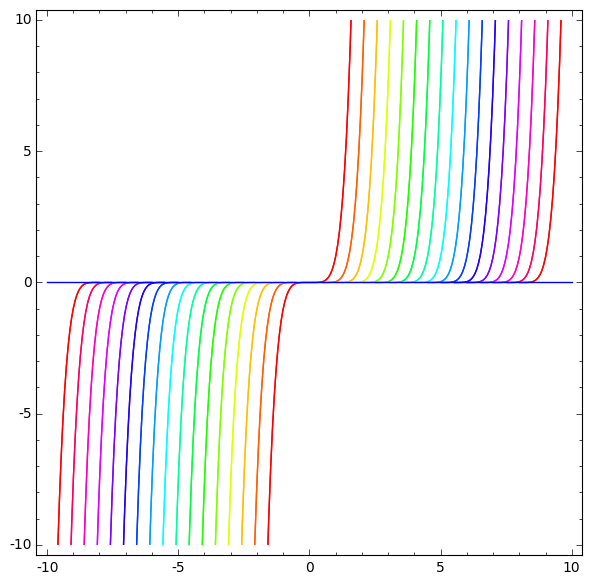
\includegraphics[width=0.6\textwidth]{plot.png}
\caption{Escoge tu color favorito.}
\end{figure}}

Por último, teniendo en cuenta que las soluciones que cumplen (PVI)$_0$ son de la forma:
$$
\begin{displaystyle}
  x(t) =
  \begin{cases}
    (t - m)^{5}, & \text{si } t \leq m \\
    0, & \text{si } m \le t \leq n \\
    (t - n)^{5}, & \text{si } n \le t
  \end{cases}
\end{displaystyle}
$$
con $m$ y $n$ variables, la primera menor que cero y la segunda mayor. Es inmediato ver que en $1$ puede tomar todos los valores en $k\in[0, 1]$ cogiendo $n = 1  - \sqrt[5]{k}$.
$\hfill \square$
}
\end{itemize}
\end{document}
